%Chapter 7

% Chapter 7 from the standard thesis template
% Conclusions and Future work
\chapter{CONCLUSION AND FUTURE WORK} \label{ch:conclusion}

\section{Conclusion}
In this thesis we have shown that a SDR-based radiometer, using off the shelf components, is able to perform comparable to a traditional radiometer.  Additionally, it was demonstrated that our SDR-based radiometer could be easily extended to mitigate radio frequency interference.   

\section{Future Work}\label{Futurework}

Two possible future work items are: 1) moving the signal processing to a dedicated processor, and 2) building more complex radiometer systems (e.g. Dicke radiometer).  These topics will be covered in the following paragraphs.   

\emph{Removing the PC.}  For this thesis, we used software that would run on a PC or comparable computer system running a full operating system such as Linux.  This allowed for rapid development by using software tools such as GNURadio to develop the SDR-based radiometer.  While this is a great platform for prototyping a SDR-based radiometer, it does require hardware that is capable of running a full operating system and the associated software.  Some radiometer applications would find this acceptable, however, other remote sensing applications (e.g. space satellite) would require a more efficient configuration.  One solution is to move the signal processing from the PC to a Field Programmable Gate Array (FPGA) or an Application-Specific Integrated Circuit (ASIC) to improve efficiency.

\emph{Implementing different types of radiometers.}  
This thesis focused on implementing a simple total power radiometer in software.  While this radiometer is effective, it relies on the fact that the components of the radiometer are stable.  Other types of radiometers have been developed that reduce this need.  

A common method is a Dicke radiometer, which was covered in this thesis.  A future work for our SDR-based radiometer would be to use a digitally generated noise source, such as a Gaussian noise source, and then switch between the antenna and this known noise source.  This noise source could also be adjusted in software, therefore stability of the noise source would not be an issue.  

{\begin{figure}[h!tb] 
\centering
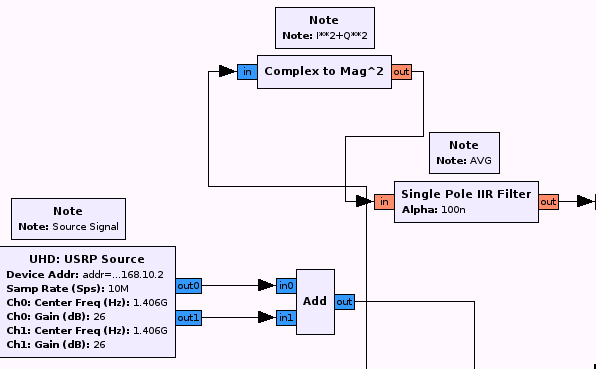
\includegraphics[width=14cm]{Images/N200_rad_corr.png}
\isucaption{A screenshot of an implementation of a correlating radiometer in GNURadio Companion.}
\label{correlating_sdr}
\end{figure}
}

Another method to improve stability and sensitivity is to correlate against a second input.  The second input could be another antenna looking at the same source, or could be two polarizations from the same antenna[\cite{Clapp}].  This results in a two receiver system looking at the same source with two signal outputs, $S_1$ and $S_2$.  Since we are looking at the same source, both signals will be correlated in time, and when multiplied they will provide an output proportional to the strength of the source signal.  The noise introduced by each receiver will then have a lower correlation due to the random nature of the noise.  This results in a radiometer with greater sensitivity due to the reduction of the noise, even though two receivers are used [\cite{Fujimoto}].

The N200 software defined radio was chosen as it is capable of having two different daughter-cards plugged in.  Therefore, it is possible to have both sources enter the software defined radio and once digitized we can sum the magnitudes of the two incoming sources.  This is easy to do and is shown in Figure \ref{correlating_sdr}.  Although Figure \ref{correlating_sdr} shows a correlating SDR-based radiometer, it has not been tested.  In theory, this should correlate the signal and improve the sensitivity of the radiometer.  Additional experimentation would be required to confirm that this implementation operates as expected.


%----------------------------------------------------------
% End of Chapter 7.  Anything below this is extra information